%:
\documentclass[11pt, oneside]{article}   	% use "amsart" instead of "article" for AMSLaTeX format
\usepackage{geometry}                		% See geometry.pdf to learn the layout options. There are lots.
\geometry{letterpaper}                   		% ... or a4paper or a5paper or ... 
%\geometry{landscape}                		% Activate for rotated page geometry
%\usepackage[parfill]{parskip}    		% Activate to begin paragraphs with an empty line rather than an indent
\usepackage{graphicx}				% Use pdf, png, jpg, or eps§ with pdflatex; use eps in DVI mode
								% TeX will automatically convert eps --> pdf in pdflatex		
\usepackage{amssymb}
\usepackage{diagbox}
\usepackage{amsmath}
\usepackage{amsthm}
\usepackage{enumerate}
\usepackage{tikz}
\usepackage{mathrsfs}
\usetikzlibrary{positioning}


\usetikzlibrary{arrows}
\theoremstyle{definition}
\newtheorem*{defn}{Definition}
\newtheorem*{prop}{Proposition}
\newtheorem*{eg}{Example}
\newtheorem*{thm}{Theorem}
\newtheorem*{corol}{Corollary}
\newtheorem{ex}{Exercise}[section]
{\theoremstyle{plain}
\newtheorem*{rmk}{Remark}
\newtheorem*{rmks}{Remarks}
\newtheorem*{lt}{Last time}
}
\newtheorem*{lem}{Lemma}
\usepackage{color}
\usepackage{CJK}
\usepackage{subfiles}
\title{Modular Domain Specifc Approaches to Efficient AGI Powered by a New Programming Language}
\author{Xiyu Zhai}
\date{}							% Activate to display a given date or no date

\begin{document}
\maketitle
\tableofcontents

\abstract {
This paper is a blueprint of a novel school of approaches to efficient AGI that is \textbf{modular} and \textbf{domain specific} and is powered by a \textbf{new programming language}. It builds upon the current success of deep learning but will outperform it in terms of sample complexity, computation efficiency (of both training and inference), explainability, robustness, accessibility to researchers and users, and ultimately the ability to evolve itself quickly and steadily.

Our insights are drawn from three a priori abstractions: \textbf{pattern recognition graph} for function approximation, \textbf{NP-ML ladder} for higher order approximation and \textbf{intelligence market} for trust and resource management. We confirm theoretically the capabilities of existing neural AI approaches under these abstractions, and then give evidence to the existence of modular domain specific approaches with better properties. The only problem is that it would take forever to implement these modular domain specific approaches using existing programming langauges. As result, a new programming language is designed with great power and novelty. It's possible to implement the new approaches in the new language primarily because it allows the implementation of \textbf{modular and domain specific machine learning algorithms beyond matrix calculation} and provides \textbf{easy visualization and timeless debugging for machine learning and even intelligence systems of scale}. An outline of the language specifications is given here, but the full details will be given in a separate paper.

We finishes by giving more details on the plans on specific domains, computer vision, natural languages, etc. The programming language is still in rapid development and these projects have yet to launch, so these details are subject to drastic change.

\section{Introduction}

\subfile{sections/introduction}

\section{Related Works}

\subfile{sections/related_works}

\section{Overview}

\subfile{sections/overview}

\section{ Pattern Recognition Graph}

\subfile{sections/pattern_recognition_graph}

\section{Higher Order Theories Based on Turing Machines}


\subfile{sections/higher_order_turing_machine}

\section{Higher Order Theories Based on Realistic Computation Models}

\subsection{Locally Sensitive Hashing}

\section{Husky Programming Language}

\subfile{sections/husky_pl}

\section{Plans for Computer Vision}

\section{Plans for Natural Language Processing}

As claimed in previous sections, deep learning's success doesn't mean it's the optimal for natural language processing, but it will serve as a convenient tool for the development of a next generation far more superior tools.

Let's first conduct a worst scenario analysis. Suppose deep learning achieved AGI before us, and the AGI works amazingly well. Let's recall what makes symbolic AI methods like expert system fail: high development, maintenance, and debugging cost. But we can instruct deep learning AGI develop expert system and write out programs that parse English like parsing a programming language. It would take forever for humans, but for AGI, it would be trivial. The takeaway is, even if deep learning takes the holy grail, it won't keep it for very long as humans could then replace it a more rule-based AI with its help.

But this argument is not satisfying, due to the gloomy prospect of deep learning achieving AGI. Still there could be many practical approaches where we can leverage deep learning in its current form to build a more advanced form of AI, which I shall explain below.

\subsection{Stage 0: Domain Specific Verifiable Natural Language Processing}

We shall restrict ourselves to a very specific domain, relatively simple, so that we can easily build up a domain specific programming langauge to describe the tasks and also build efficient solvers for the task.
\begin{center}
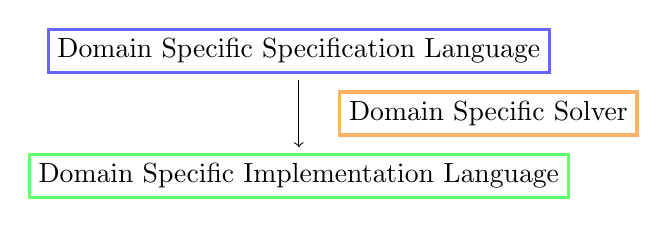
\begin{tikzpicture}[
squarednode1/.style={rectangle, draw=blue!60, fill=white!5, very thick, minimum size=4mm},
squarednode2/.style={rectangle, draw=green!60, fill=white!5, very thick, minimum size=4mm},
squarednode3/.style={rectangle, draw=orange!60, fill=white!5, very thick, minimum size=4mm},
]
%Nodes
\node[squarednode1]      (dssl)                              {Domain Specific Specification Language};
\node[squarednode2]      (dsil)              [below=of dssl]  {Domain Specific Implementation Language};

%Lines
\draw[->, shorten >=2pt, shorten <=2pt] (dssl.south) -- (dsil.north) node[squarednode3, midway, right, xshift=5mm] {Domain Specific Solver};
\end{tikzpicture}
\end{center}

\begin{eg}
	[Mathematica]
\end{eg}

\begin{eg}
	[Html, Css] Html and Css are not specification languages, they are implementation languages.
\end{eg}

Let's compare the pros and cons with ChatGPT

Here's a nice summary in table \ref{comparison} written by the very ChatGPT itself.

\begin{table}[ht]
\label{comparison}
\centering
\small % reduce font size
\begin{tabular}{|l|p{6cm}|p{6cm}|}
\hline
 & \textbf{ChatGPT} & \textbf{DSLs} \\
\hline
\textbf{Pros} & 
Flexibility: ChatGPT can be used for a wide variety of NLP tasks, including text generation, question answering, summarization, and more.
&
Increased productivity: DSLs are designed to be easy to use and understand within a specific domain, which can increase developer productivity. \\
\cline{2-3}
& 
Ease of use: ChatGPT can be accessed through simple API calls or integrated into other applications and platforms.
&
Enhanced control: A DSL provides more fine-grained control over a specific problem within a domain, allowing developers to tailor their solutions to specific requirements. \\
\cline{2-3}
& 
Low development time: Implementing a ChatGPT-based solution typically requires less development time than creating a custom DSL.
&
Improved maintainability: DSLs can make code more readable and maintainable within a specific domain, as they typically use domain-specific terminology and concepts. \\
\cline{2-3}
& 
Multilingual support: ChatGPT can generate text in multiple languages.
&
 \\
\hline
\textbf{Cons} & 
Limited control: ChatGPT generates text based on its training data and can sometimes produce unexpected or incorrect output.
&
Higher development time: Developing a custom DSL can require a significant amount of time and effort. \\
\cline{2-3}
& 
Lack of transparency: It can be difficult to understand why ChatGPT generates a particular piece of text, making it hard to debug or fine-tune.
&
Limited flexibility: A DSL is designed to solve a specific problem within a specific domain, so it may not be suitable for other tasks or domains. \\
\cline{2-3}
& 
Dependence on data quality: The quality of ChatGPT's output is heavily dependent on the quality and diversity of its training data.
&
Steep learning curve: Developers may need to learn a new syntax and programming paradigm in order to use a DSL effectively. \\
\hline
\end{tabular}
\caption{Comparison of ChatGPT and DSLs}
\label{tab:chatgpt-dsls}
\end{table}

I'm sorry that I have to copy because my hands are not in 100\% health.

\clearpage

We could have the best of both worlds by combining dsls with deep learning like this:
\begin{center}
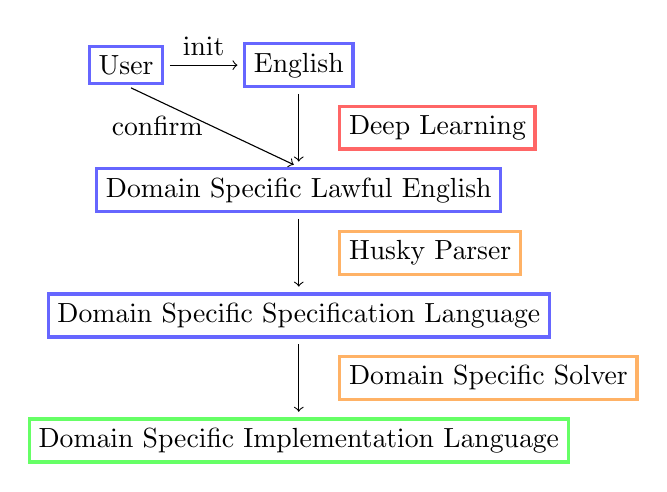
\begin{tikzpicture}[
squarednode1/.style={rectangle, draw=blue!60, fill=white!5, very thick, minimum size=4mm},
squarednode2/.style={rectangle, draw=green!60, fill=white!5, very thick, minimum size=4mm},
squarednode3/.style={rectangle, draw=orange!60, fill=white!5, very thick, minimum size=4mm},
squarednode4/.style={rectangle, draw=red!60, fill=white!5, very thick, minimum size=4mm},
]
%Nodes
\node[squarednode1]              (user)                              {User};
\node[squarednode1]      (e)             [right=of user]   {English};
\node[squarednode1]      (dsle)             [below=of e]   {Domain Specific Lawful English};
\node[squarednode1]      (dssl)             [below=of dsle]    {Domain Specific Specification Language};
\node[squarednode2]      (dsil)              [below=of dssl]  {Domain Specific Implementation Language};

%Lines
\draw[->, shorten >=2pt, shorten <=2pt] (user.east) -- (e.west) node[midway, above] {init};
\draw[->, shorten >=2pt, shorten <=2pt] (user.south) -- (dsle.north) node[midway, left] {confirm};
\draw[->, shorten >=2pt, shorten <=2pt] (e.south) -- (dsle.north) node[squarednode4, midway, right, xshift=5mm] {Deep Learning};
\draw[->, shorten >=2pt, shorten <=2pt] (dsle.south) -- (dssl.north) node[squarednode3, midway, right, xshift=5mm] {Husky Parser};
\draw[->, shorten >=2pt, shorten <=2pt] (dssl.south) -- (dsil.north) node[squarednode3, midway, right, xshift=5mm] {Domain Specific Solver};
\end{tikzpicture}
\end{center}

First, we create a subset of English called Domain Specific Lawful English such as
\begin{enumerate}[(i)]
	\item it's grammarly and semantically rigorous, so that parsing in Husky code is feasible (although it might be too difficult for traditional languages like C++/Rust/Python/Haskell)
	\item it's expressive enough for the domain and can be faithfully translated into the Domain Specific Specification Language
	\item easily understood by users
\end{enumerate}

Second, we collect data and train a deep neural network that can translate arbitrary English into the subset.

When user initializes a dialogue using arbitrary English, it's translated into Domain Specific Lawful English, which is checked by the Husky Parser and also confirmed by the user that the translation is correct.

Then the Domain Specific Lawful English is translated by the Husky Parser into Domain Specific Specification Language so that it's acceptable by the solver.

Obviously, this setup will have the advantages of both worlds.

The details will be covered in the followup papers.

\subsection{Stage 1: Universal Lawful English}

Todo

\subsection{Stage 2: Minimizing Usage of Deep Learning}

Todo

\subsection{Stage 3: Learning Augmented Verifiable Solver}

Todo

\subsection{Stage 4: Generating Human Readable Explanations}

Todo

\end{document}